\documentclass{beamer}
\usepackage[utf8]{inputenc}
\usepackage{default}
% \usepackage{geometry}
% \usepackage{enumitem}
% \setlist{align=left}
\usetheme{Antibes}
\geometry{paper=a4}

\title{Patena : Herramienta para diseño racional de secuencias linker}
\date{5 Junio - 2015}

\begin{document}

\begin{frame}
 \titlepage
\end{frame}

\section{Introducción}

\begin{frame}{Linkers naturales}
 No tan simples de definir/describir/clasificar
 \begin{itemize}
  \item Hay flexibles y rígidos    %VER MOLECULAR RULERS
  \item Función extra: mutaciones/deleciones pueden suprimir la actividad    %FORMAN PARTE DE LA FUNCIÓN DE LA PROTEINA O SE MANTIENEN INERTES? QUIZAS NO ESTÉN EN EL DOMINIO PERO PUEDEN AYUDAR A LA ESTRUCTURA, A UNIR LIGANDOS?? A QUE MAS??
%   PUEDE MOSTRAR UNA FUNCION EN UN CIERTO CONTEXTO EXPERIMENTAL DISTINTO AL NATURAL !!!!  
  \end{itemize}
 
\end{frame}

\begin{frame}{Objetivo}
Obtener secuencias linker que puedan ser usadas experimentalmente 
para ingeniería de proteinas. Ejemplo: 
\begin{itemize}
 \item Formación de proteinas bifuncionales mediante union covalente de dominios.
 \item Promover la unión entre proteinas que forman complejos, generando una unión covalente entre ellos
\end{itemize}

Requiere:
\begin{itemize}
 \item Estructura flexible
 \item Inerte
\end{itemize}
Disponible actualmente: Búsquedas en bases de datos
\end{frame}


% \end{frame}
% \begin{frame}{Herramientas disponibles para elegir linkers}

\begin{frame}{Fundamentos}
 \begin{itemize}
  \item Existen diversas herramientas disponibles para evaluar propiedades estructurales y funcionales a partir de la secuencia.
  \item Existe un valor target para estas herramientas 
  \item El número de secuencias favorables es considerablemente 'amplio' con respecto al espacio de posibles soluciones.
 \end{itemize}
%  La solución es una secuencia tal que las herramientas de evaluación predigan propiedades inertes y no estructuradas.
\end{frame}


% ACLARAR QUE TODAS LAS HERRAMIENTAS SE BASAN EN LA BÚSQUEDA DE PROPIEDADES EXLUSIVAMENTE A PARTIR DE LA SECUENCIA DE AAs

\section{Esquema para buscar una solución}

\begin{frame}{Solución planteada}
\begin{itemize}
 \item Iniciamos la búsqueda mediante una secuencia random o definida por el usuario. Es solo un punto de partida!
 \item Definimos un mecanismo de score por posición en función del resultado de las herramientas:
    Menor score = mejor solución  
 \item Mutamos y reevaluamos iterativamente la secuencia inicial, en búsqueda de score mínimo(0). 
 \item Las mutacione son aceptadas heurísticamente siguiendo un método de Monte Carlo, guiado por el score global (suma de puntajes de todas posiciones de la secuencia).
\end{itemize}
\end{frame}

\begin{frame}
 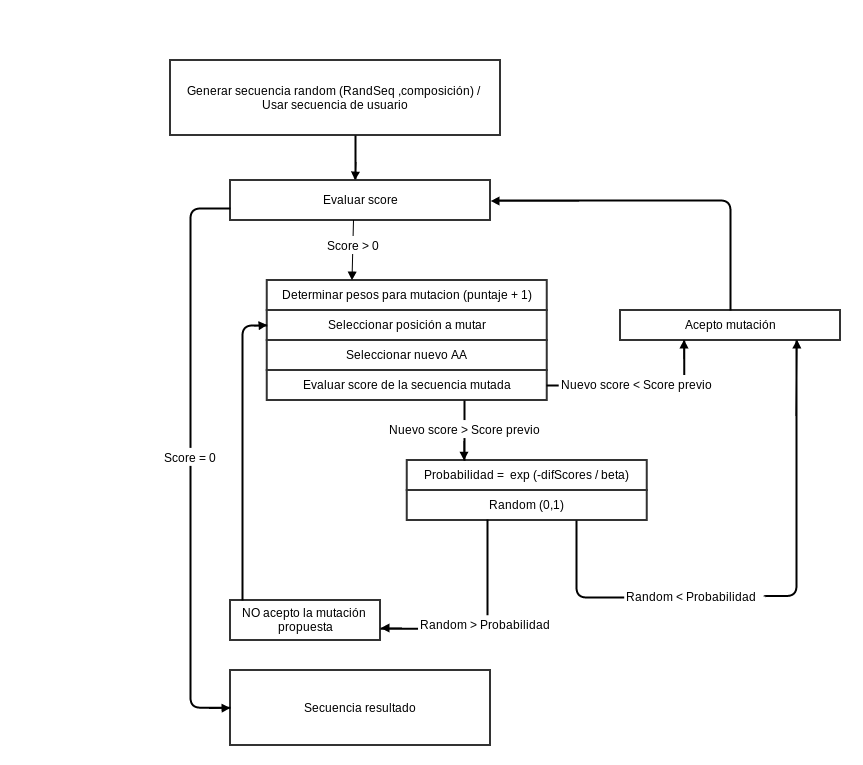
\includegraphics[width=\textwidth,height=\textheight]{esquemaGeneral.png}
\end{frame}



\section{Herramientas de evaluación}

% \subsection
\begin{frame}{Herramientas ya implementadas}
%  ESTAN SON LAS QUE YA EXPLIQUE LA VEZ PASADA
\begin{description}[]
%   \begin{itemize}
   \item[IUPred:] Predicción de conformación definida 
   \item[ANCHOR:] Predicción de proteinas que adoptan estructuras al unirse a otras. 
   \item[BLAST:] Funcionalidad mediante homología secuencial  
   \item[ELM:] Principales módulos funcionales encontrados en regiones intrínsecamente desordenadas.
   \item[Prosite:] Motivos lineales que podrían estar asociados a funciones.
%    \end{itemize}
\end{description}

\end{frame}


\subsection{Nuevas herramientas incorporadas}

\begin{frame}{Tango}
El método se deriva a partir de aplicar la mecánica estadística a un conjunto de datos 
experimentales obtenidos de los residuos en de proteinas que promueven la formacion de amyloids. 

Resulta en una probabilidad de cada residuo a adoptar cierta conformación:
\\[2ex]
\begin{tabular}[h]{c| c| c| c| c| c| c}
res & aa & Beta &Turn &	Helix	& Aggregation &	Conc-Stab\_Aggregation \\
01 &	L	&3.5&	 0.0&	0.000&	0.000 &	0.000\\ 

\end{tabular}
\end{frame}


\begin{frame}{Waltz}  
  \begin{itemize}
   \item Determinantes secuenciales de la formación de amyloids
   \item Utiliza una PSSM derivada de información secuencial y propiedades fisicoquímicas y estructurales. 
  \end{itemize}

\end{frame}

\begin{frame}{Limbo}  
  \begin{itemize}
   \item Predice sitios de unión a chaperonas (heptapéptidos) 
   \item Información de estudios secuenciales(ensayos de binding)
   \item Parámetros estructurales obtenidos de modelado por homología. Structural parameters from homology modelling
   \item Evaluación = aplicar una matriz de scores. 
   \item Resultado=scores por posición. Importancia del threshold
  \end{itemize}

\end{frame}

\begin{frame}{Determinantes secuenciales para formación de Amyloids}  
 Determinados a partir de un conjunto de péptidos cortos sintetizados y evaluados experimentalmente.
 
 A pH Neutral:
 
 ${P}_1 - {PKRHW}_2 -[VLS(C)WFNQ]_3 -[ILTYWFN]_4 - [FIY]_5- {PKRH}_6$
\end{frame}

\begin{frame}{Secuencias transmembrana}
 \begin{itemize}
  \item TMHMM Server v. 2.0
  \item Usado como clasificador binario: transmembana o no
 \end{itemize}

\end{frame}


\begin{frame}{Pasta}
Predicción de agregación amiloide
\begin{itemize}
 \item Asume que las interacciones en la formación de estructuras cross-beta(estructura asociada a fibras amiloides) es el mismo que ocurre en las estructuras de hoja plegada beta.
 \item Utiliza un conjunto de datos de estructuras conocidas para derivar un potencial estadístico de interacción entre cada par posible de AAs en este tipo de estructura.
 \item Durante la evaluación, el algoritmo utiliza este potencial para evaluar todos los posibles emparejamientos de la secuencia input con si misma, tanto paralela como antiparalelamente.
 \item El emparejamiento que tenga menor energia asignada se predice como el que se adopará en caso que se forme el agregado de tipo amiloide.
\end{itemize}

 
\end{frame}

\begin{frame}{Pasta}	
 \includegraphics[width=\textwidth,height=0.9\textheight]{pastaExample.pdf}
\end{frame}

% \begin{frame}{Pasta}	
% 
% *************************************
% Starting PASTA evaluation
% Threshold: 0.1
% Hit:
% Positions:    1-4
% RESULTS:
% M|V|L|S|P|A|D|K|T|N|V|K|A|A|W|G|K|V|G|A|H|A|G|E|Y|G|A|E
% 1|1|1|1|1|0|0|0|0|0|0|0|0|0|0|0|0|0|0|0|0|0|0|0|0|0|0|0
% Hit enter to continue with next evaluation
% 
% \end{frame}

% \subsection
\begin{frame}{Otras funcionalidades}
 \begin{itemize}
  \item Carga neta de la secuencia
  \item Secuencias flanqueantes estáticas
  \item Distintas opciones de ejecución: full verbose,silent, limite de iteraciones, deshabilitar herramientas puntuales
 \end{itemize}
\end{frame}

\section{Ejemplo}
\begin{frame}{Evaluación}
 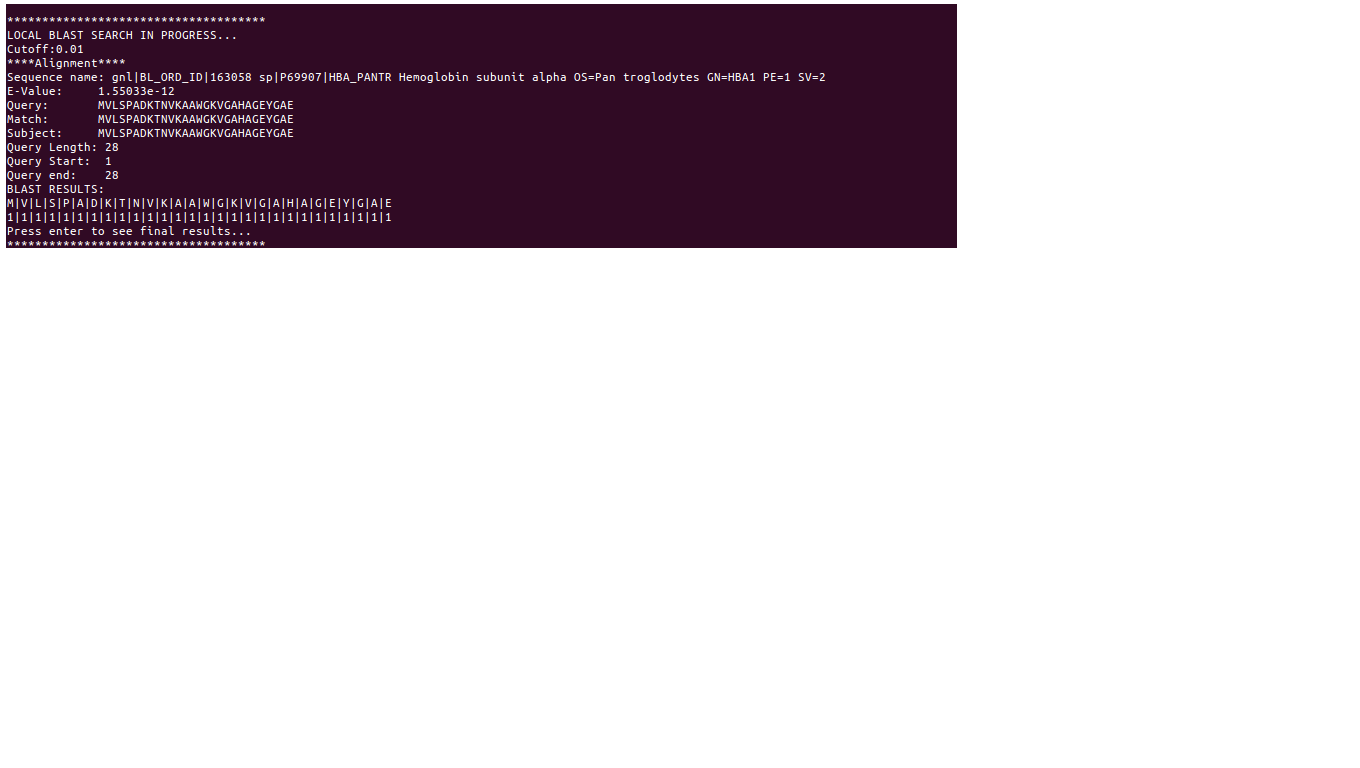
\includegraphics[width=1.7\textwidth,height=2.2\textheight]{blastExample.png}
\end{frame}

\begin{frame}{Propuesta de mutación}
 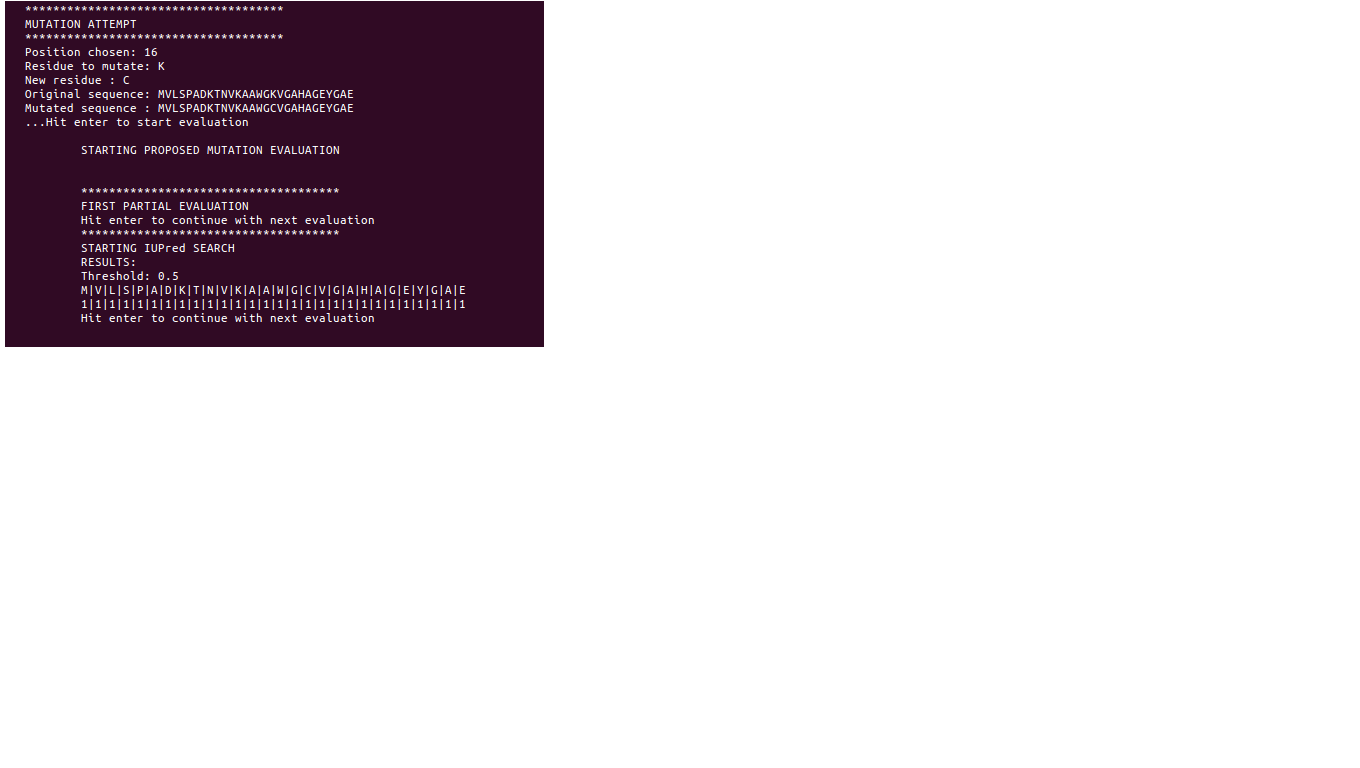
\includegraphics[width=2.4\textwidth,height=1.9\textheight]{mutAttempt.png}
\end{frame}

\begin{frame}{Decisión}
 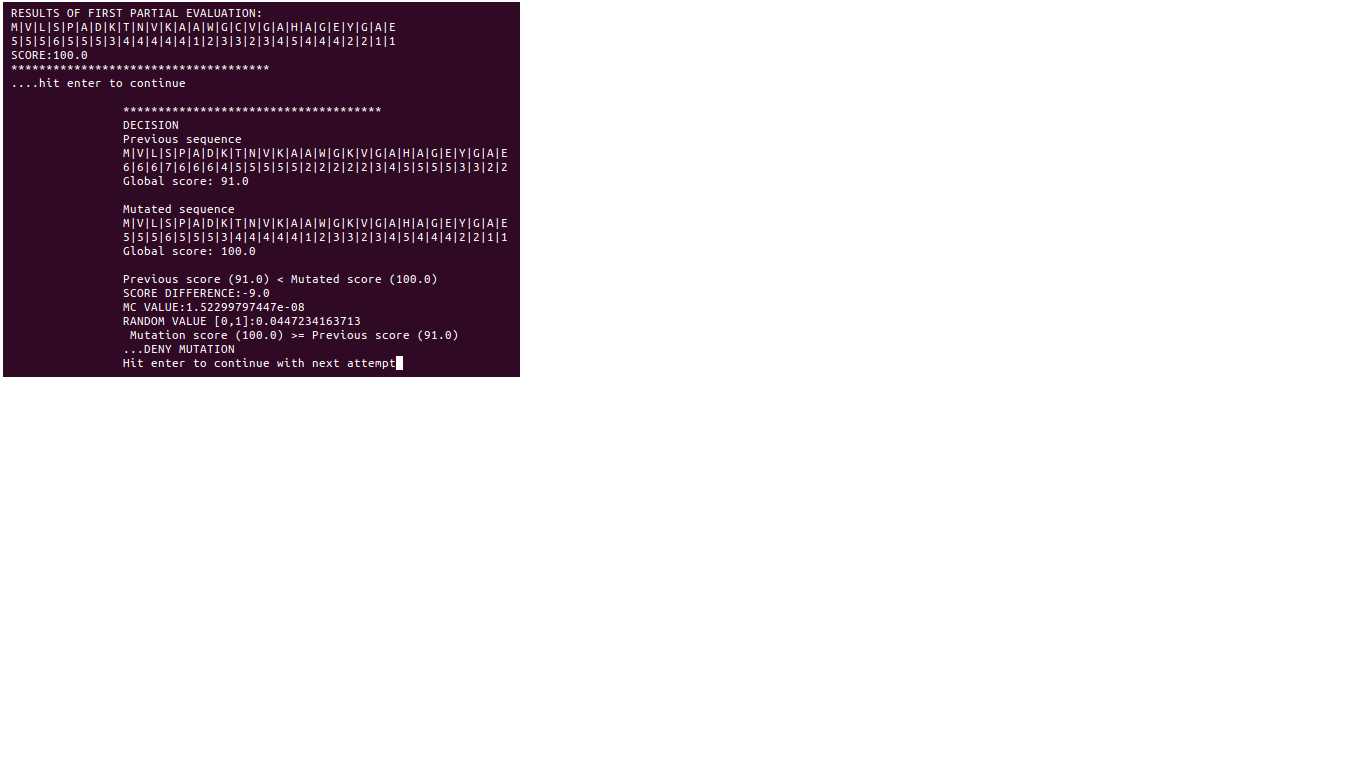
\includegraphics[width=2.4\textwidth,height=1.9\textheight]{decision.png}
\end{frame}


\section{Resultados}
% \begin{frame}{Tests}
 
% \end{frame}

\begin{frame}{Tiempo de ejecución - Beta = 1.0}
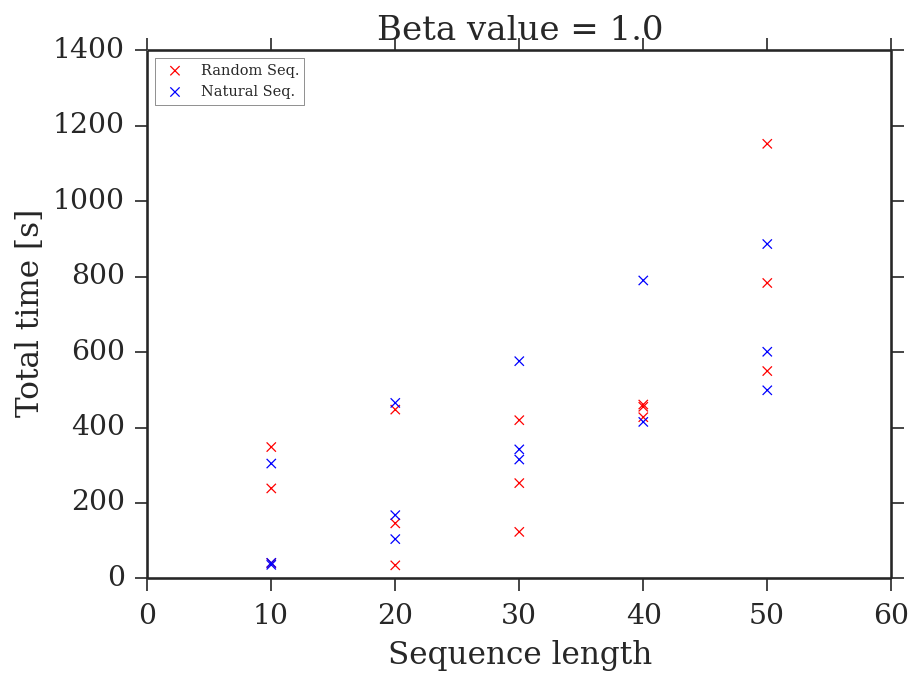
\includegraphics[width=\textwidth,height=0.8\textheight]{largo-beta.png}
\end{frame}


\begin{frame}{Tiempo de ejecución - Seq = 30}
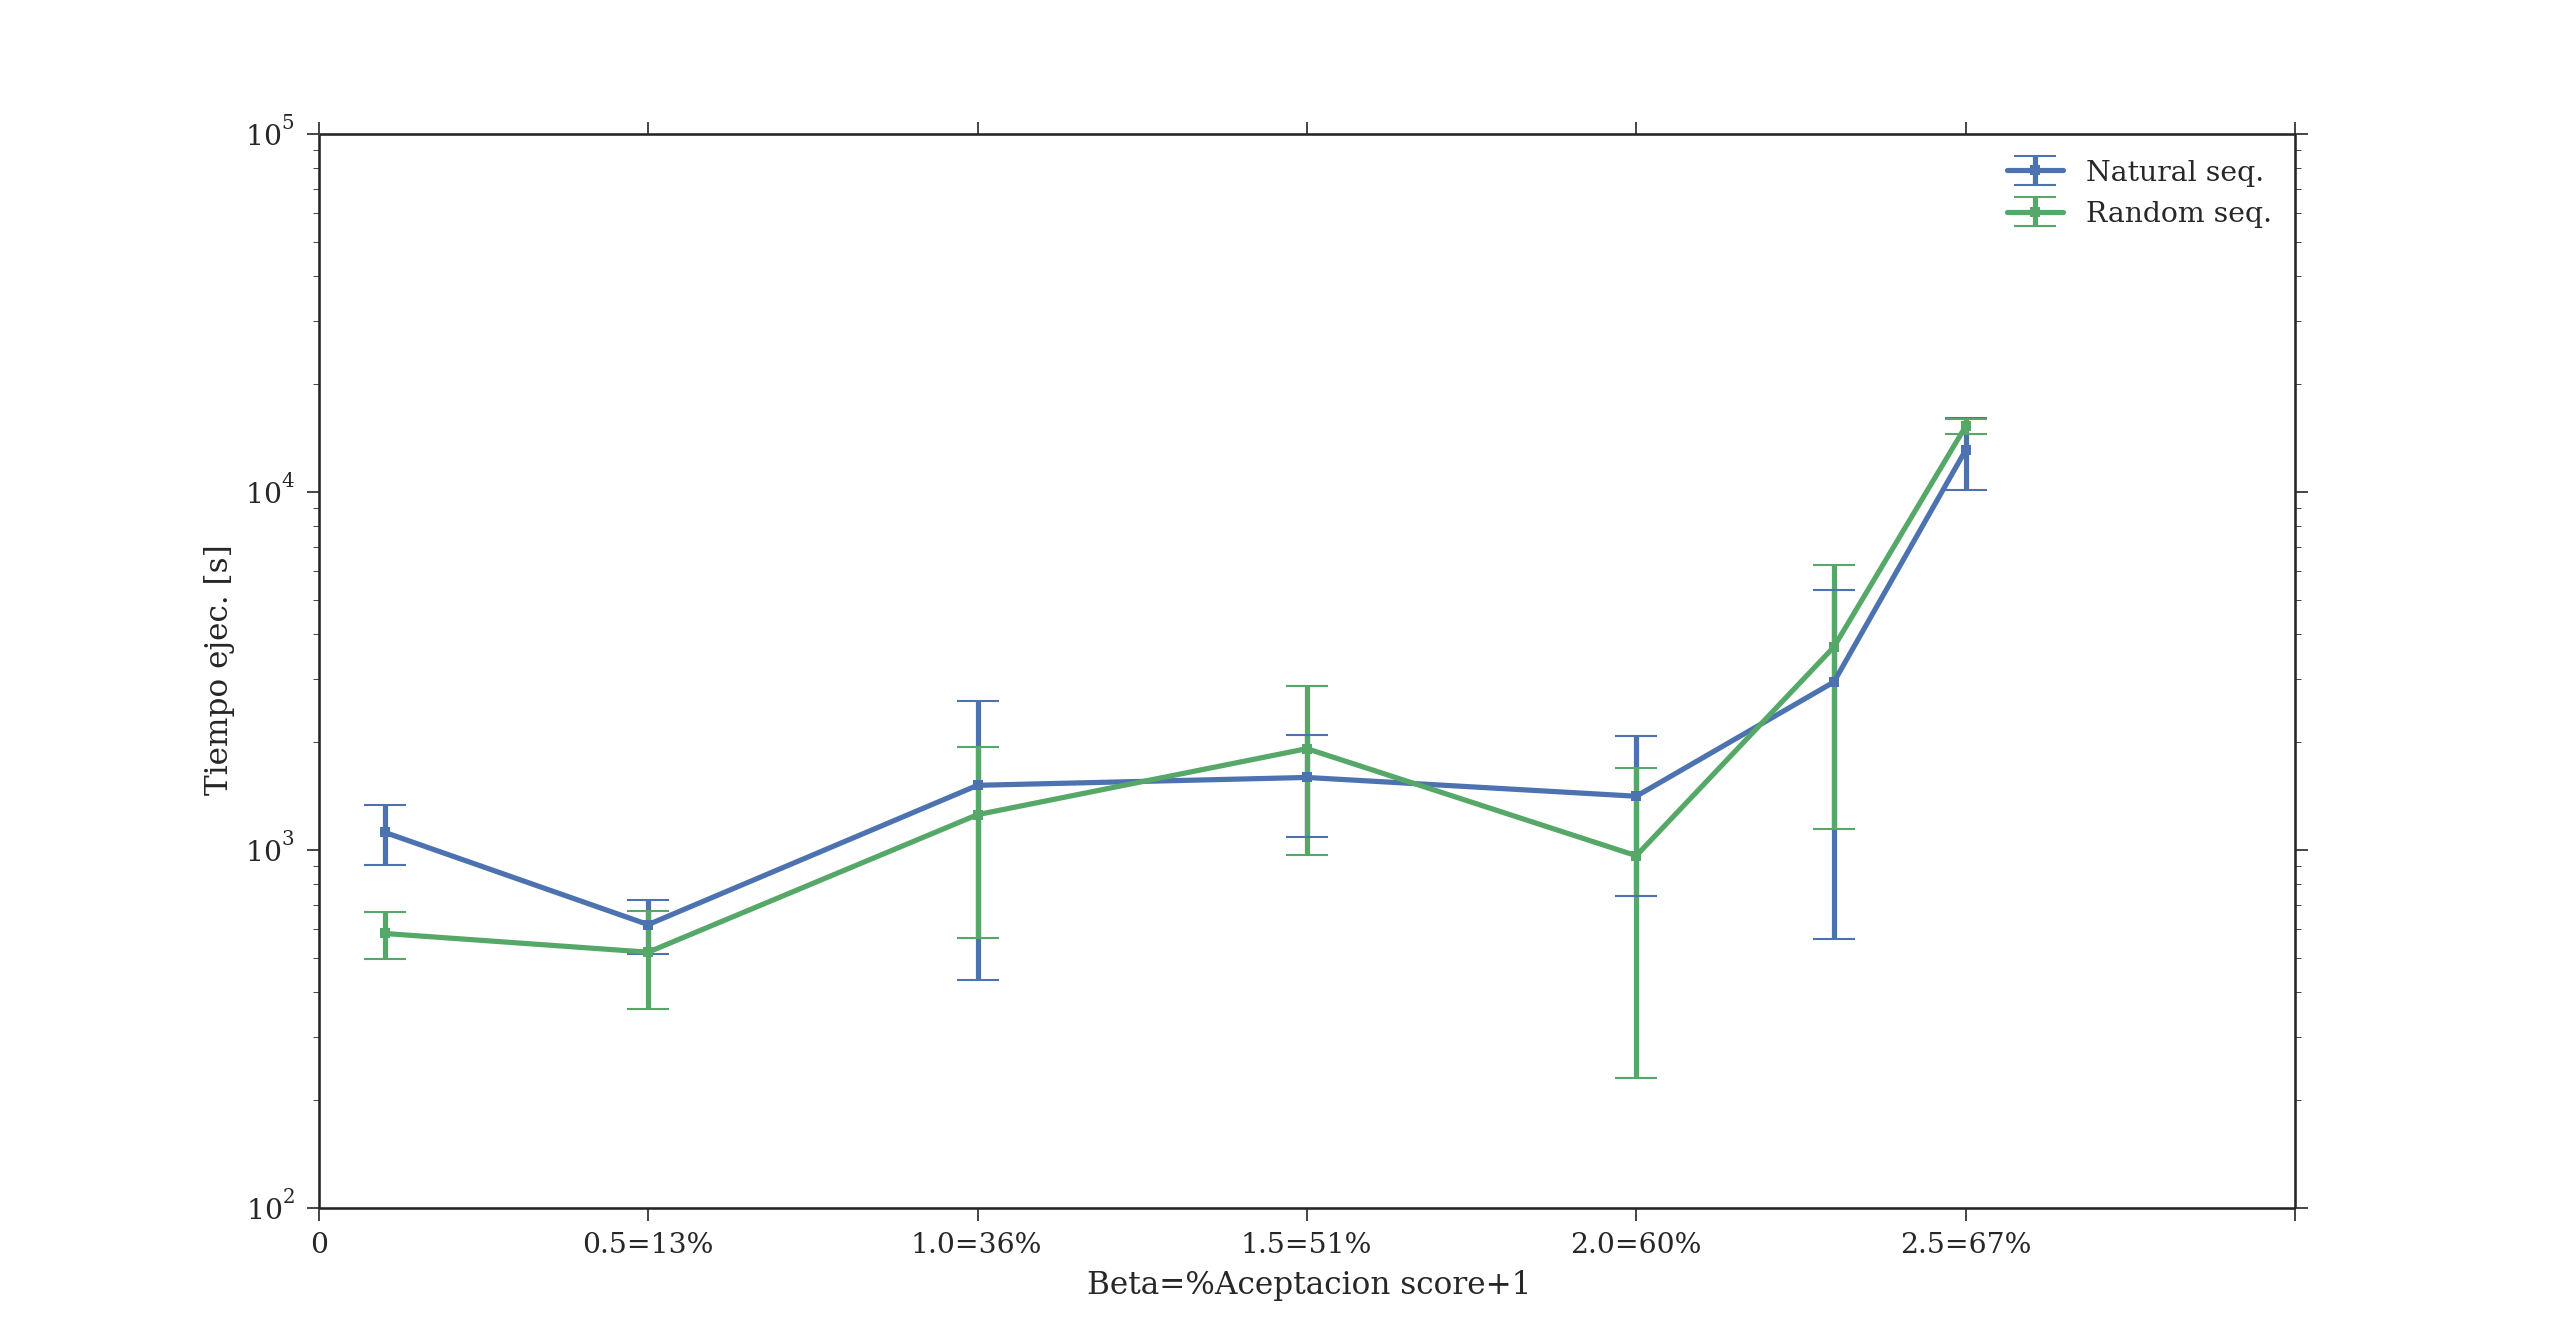
\includegraphics[width=\textwidth,height=0.85\textheight]{beta-time.png}
\end{frame}

\begin{frame}{Intentos de mutación - Seq = 30}
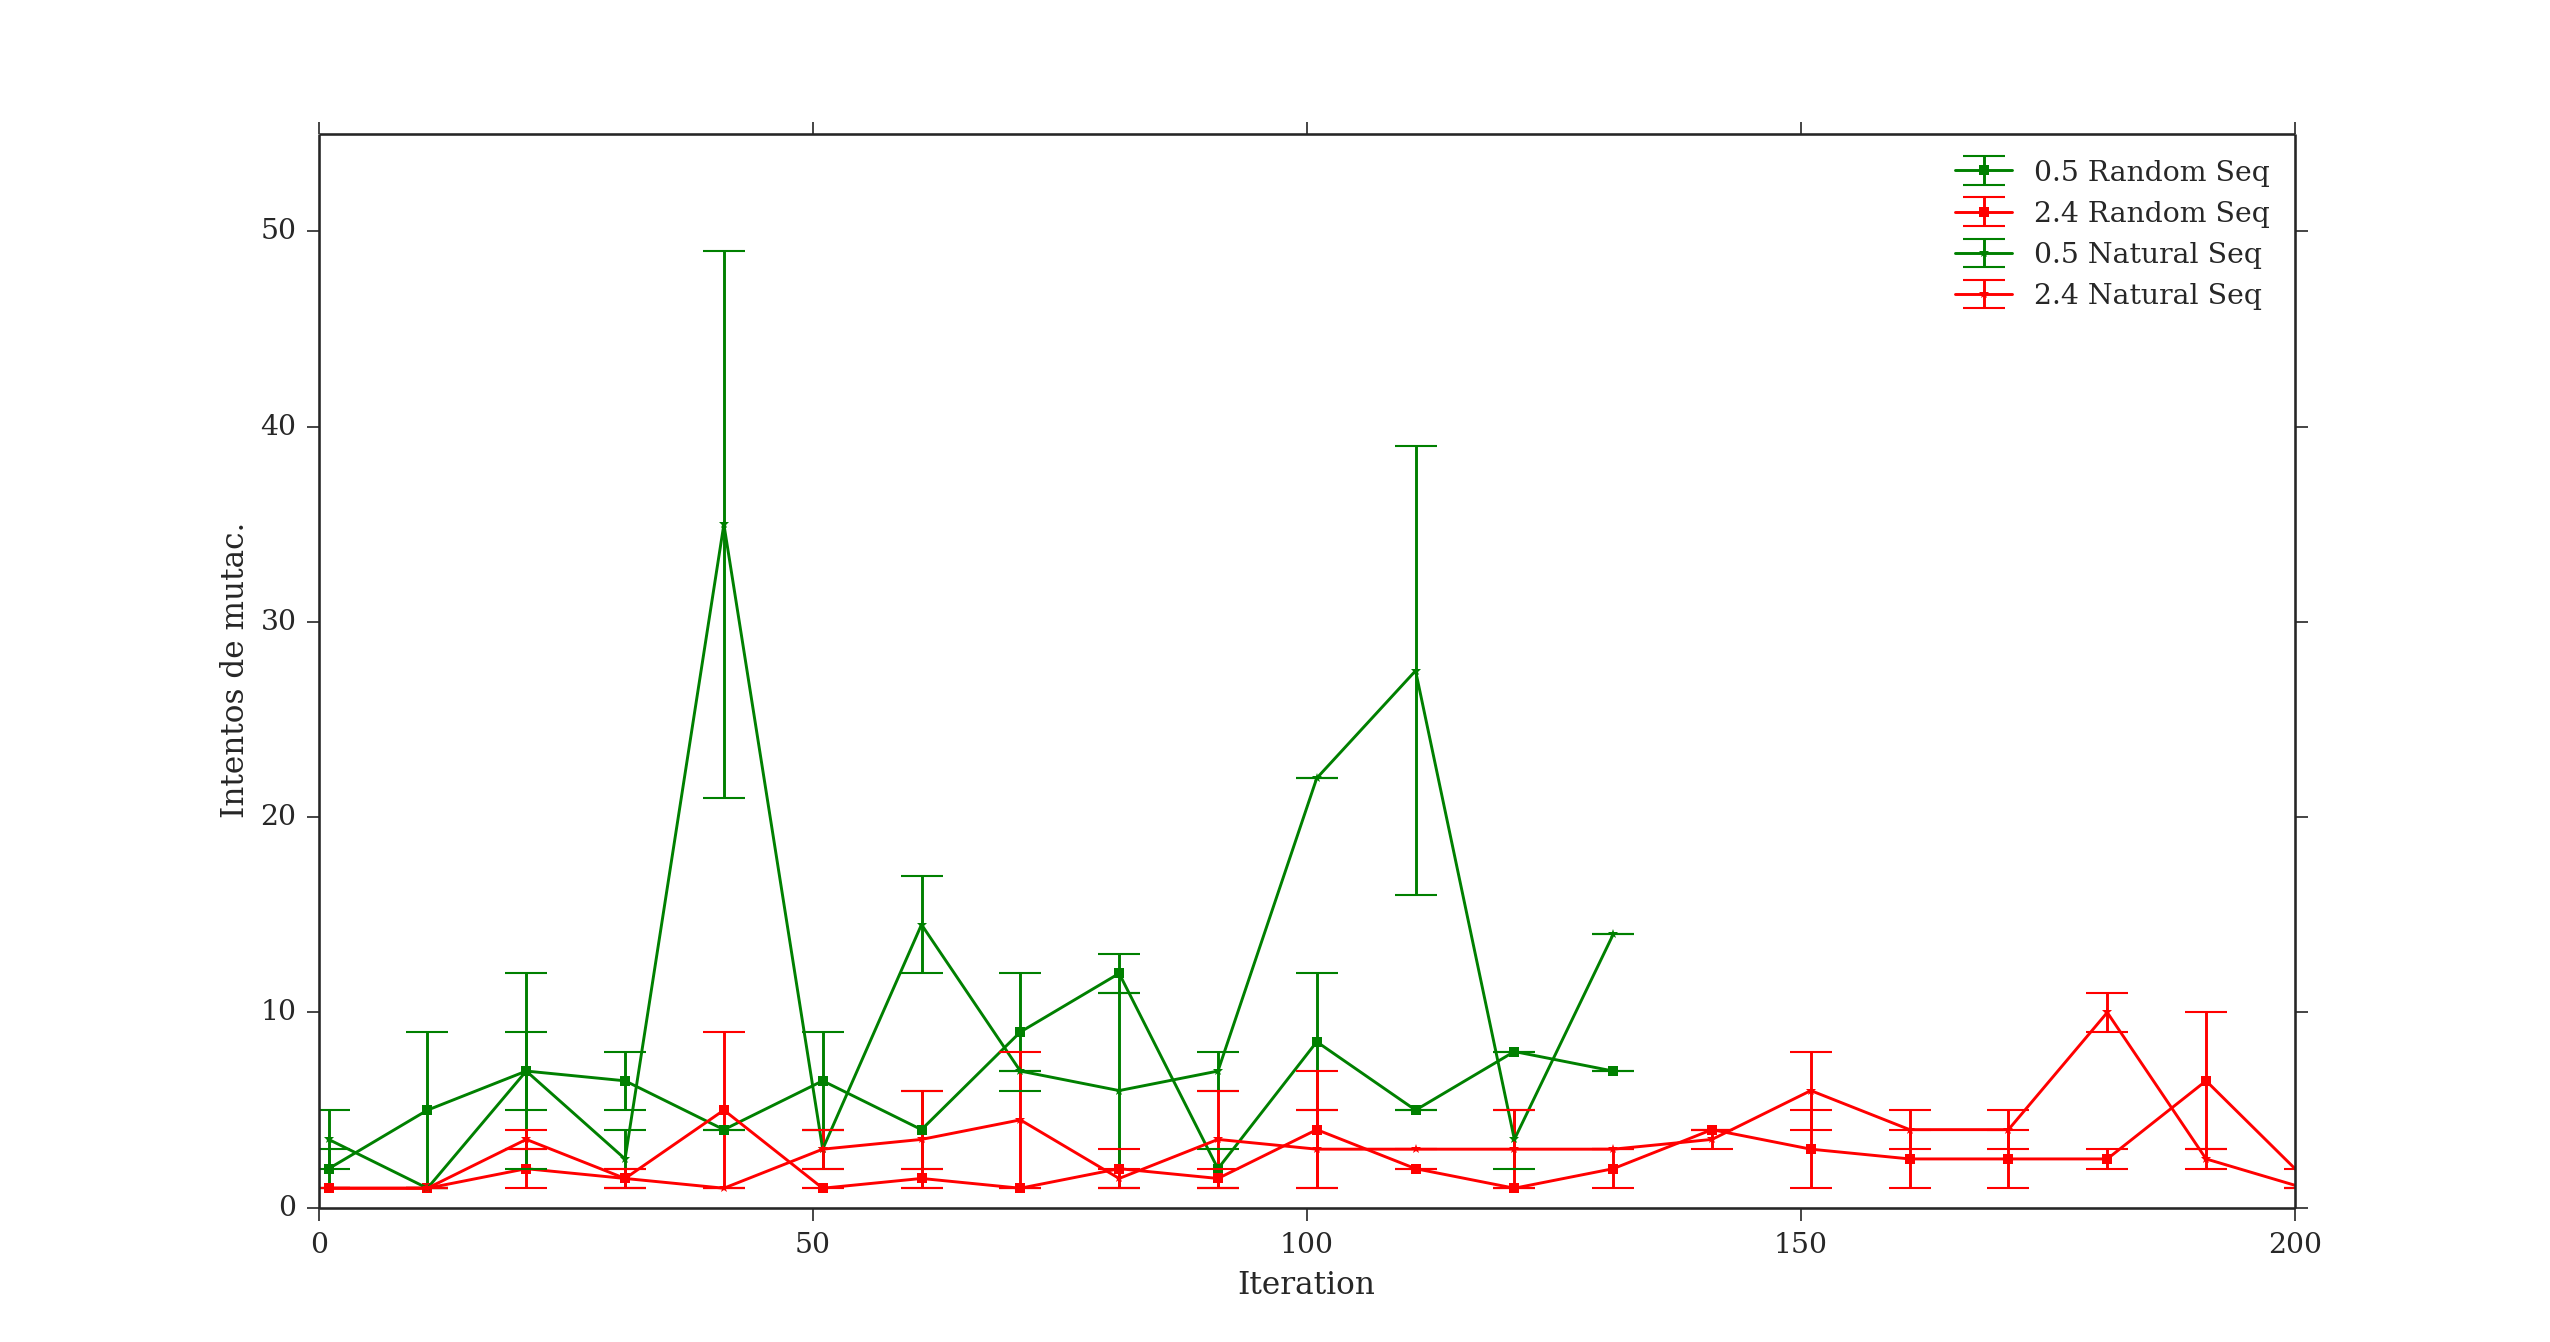
\includegraphics[width=\textwidth,height=0.85\textheight]{mutAttempts.png}
\end{frame}

\begin{frame}{Intentos de mutación - Corridas individuales - Seq = 30}
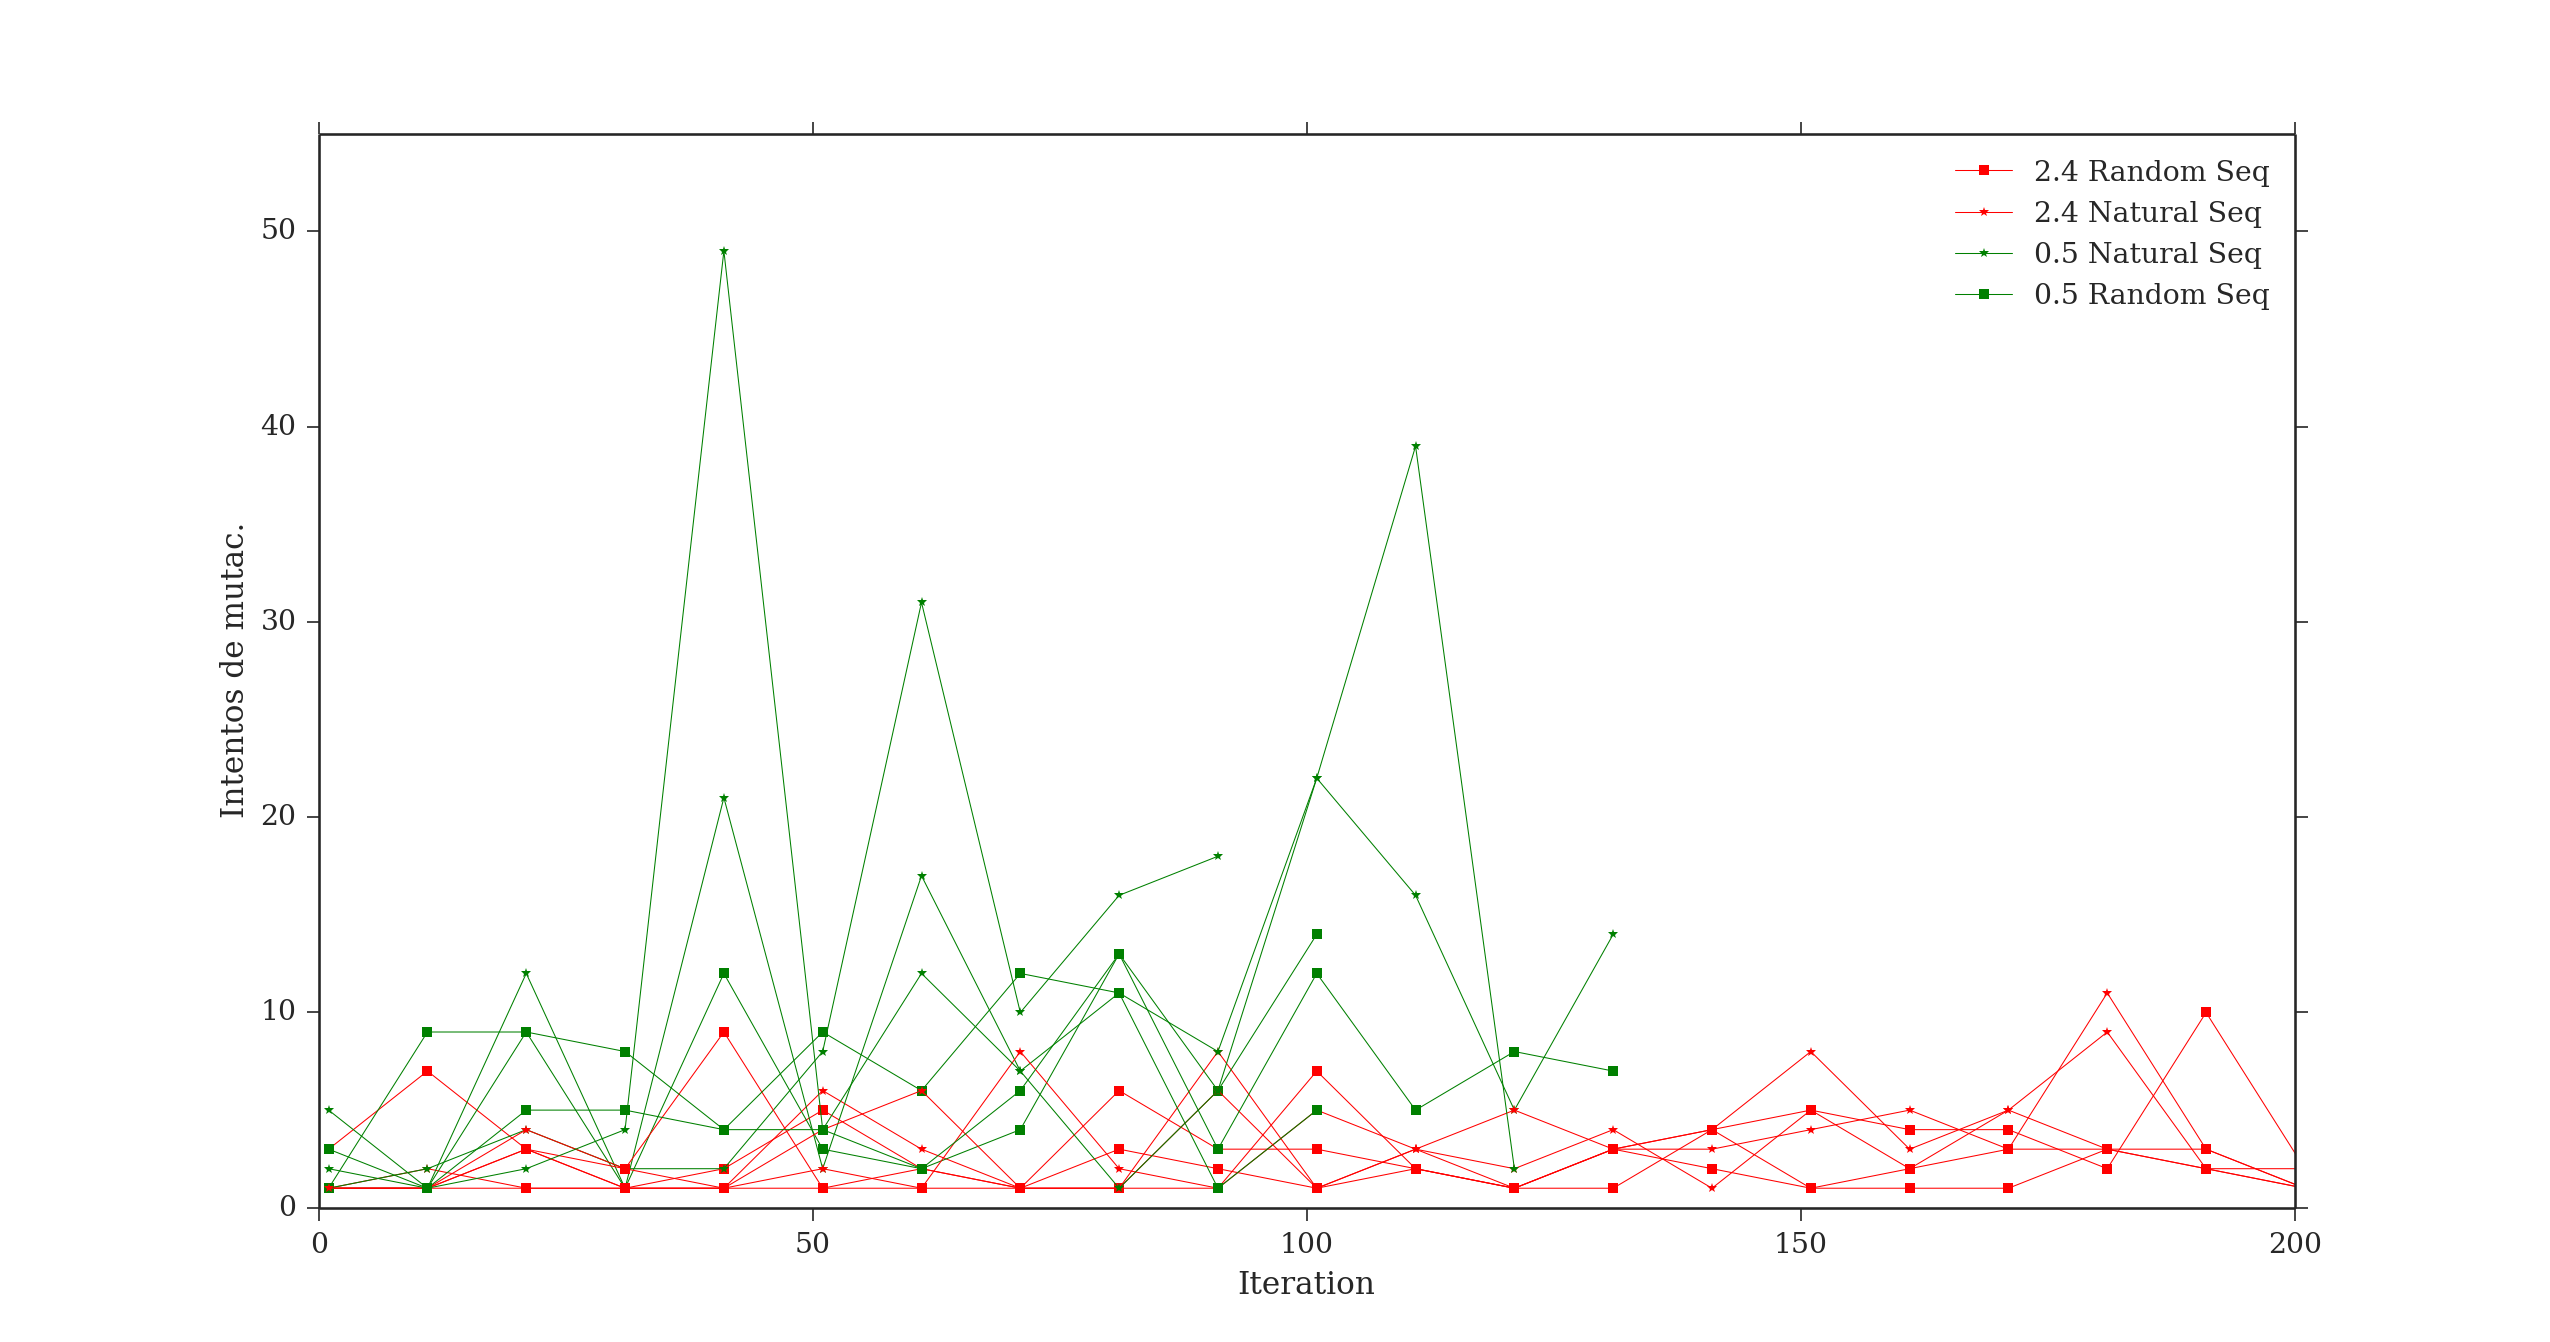
\includegraphics[width=\textwidth,height=0.85\textheight]{mutAttemptsRuns.png}
\end{frame}

\begin{frame}{Intentos de mutación - Corridas individuales - Seq = 30}
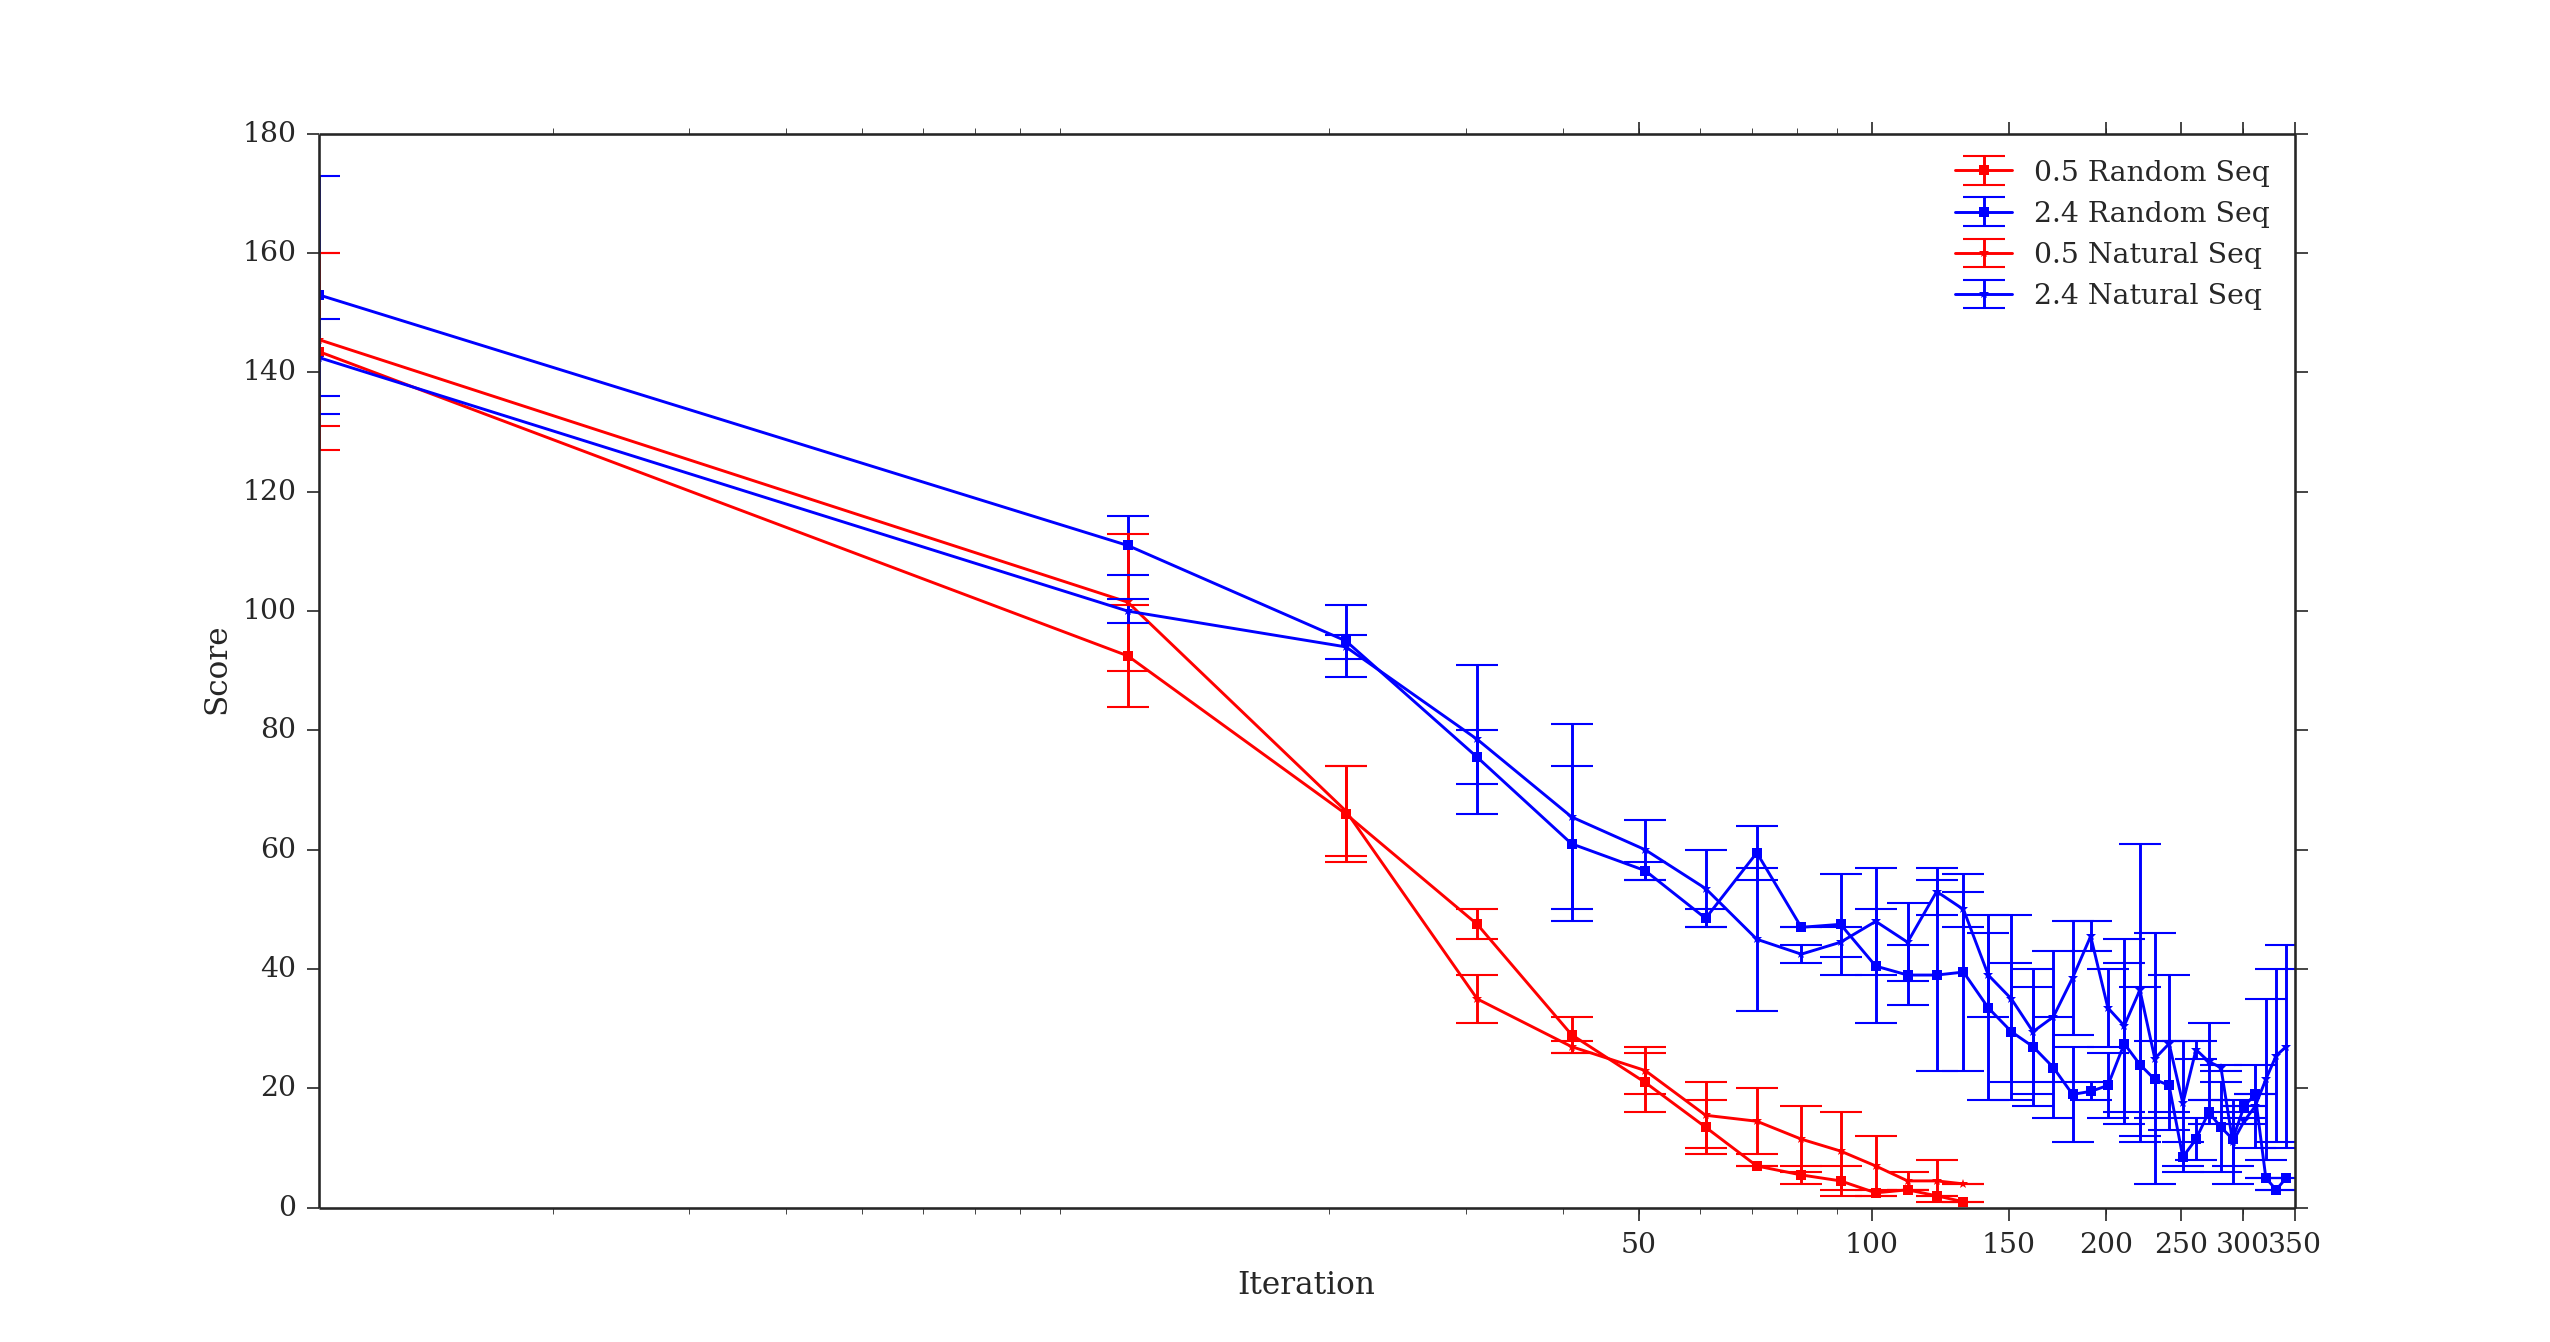
\includegraphics[width=\textwidth,height=0.85\textheight]{scoreVsIterMean.png}
\end{frame}


\begin{frame}{Secuencia inicial constante - Divergencia de las ejecuciones}
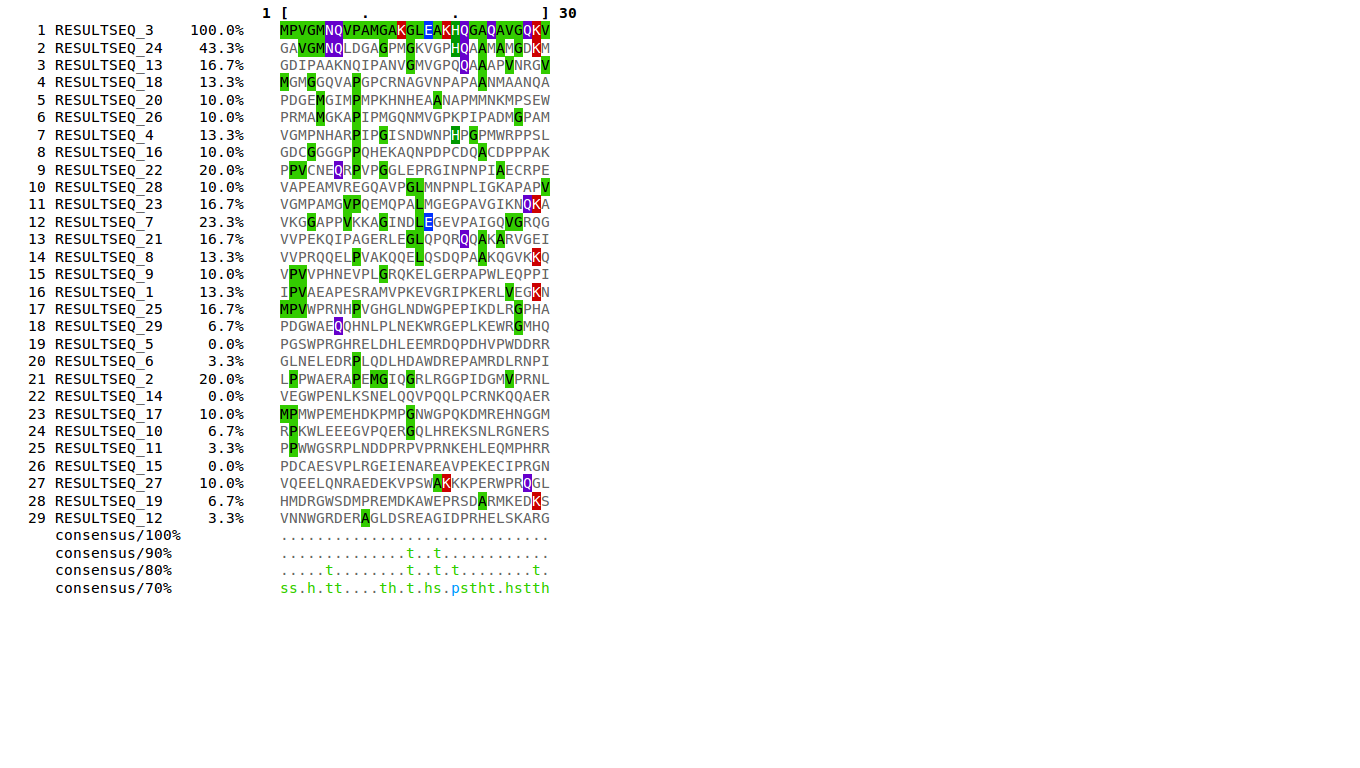
\includegraphics[width=1.5\textwidth,height=1.1\textheight]{divergencia.png}
\end{frame}

\section{A futuro}

\begin{frame}{Queda por hacer}
\begin{itemize}
\item Agregar/actualizar herramientas de evaluación, refinar los parámetros de éstas. 
\item Incorporar las secuencias generadas a una base de datos. 
%DE ESTA FORMA, DESPUES SE PUEDE ARMAAR UNA FUNCIONALIDAD QUE 
% ADEMAS, UNA VEZ QUE SE TIENE UNA BD CON UNA CANTIDAD CONSIDERABLE DE SECUENCIAS SE PUEDE  USAR COMO BASE PARA DIFERENTES ESTUDIOS 
\end{itemize}
\end{frame}	

\end{document}
